\documentclass[a4paper,12pt]{article}

\usepackage{tikz}
\usepackage{amsmath}
\usepackage{gensymb}

\usetikzlibrary{arrows.meta}

\begin{document}

\begin{figure}[h]
\centering
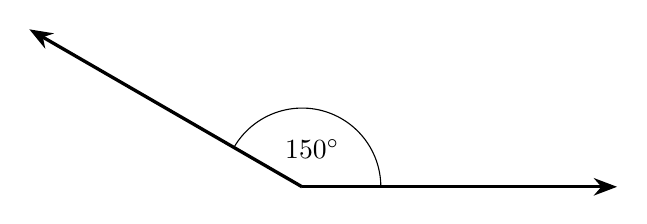
\begin{tikzpicture}[rotate=0]
\draw[very thick,-Stealth] (0,0) -- (150:4);
\draw[very thick,-Stealth] (0,0) -- (0:4);
\draw (150:1) arc[radius=1,start angle=150,end angle=0];
\path (75:0.5) node{$150\degree$};
\end{tikzpicture}
\end{figure}

\begin{figure}[h]
\centering
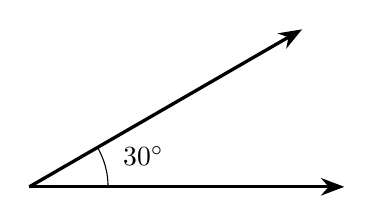
\begin{tikzpicture}[rotate=0]
\draw[very thick,-Stealth] (0,0) -- (30:4);
\draw[very thick,-Stealth] (0,0) -- (0:4);
\draw (30:1) arc[radius=1,start angle=30,end angle=0];
\path (15:1.5) node{$30\degree$};
\end{tikzpicture}
\end{figure}

\begin{figure}[h]
\centering
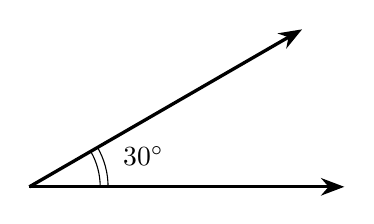
\begin{tikzpicture}[rotate=0]
\draw[very thick,-Stealth] (0,0) -- (30:4);
\draw[very thick,-Stealth] (0,0) -- (0:4);
\draw (30:1) arc[radius=1,start angle=30,end angle=0];
\draw (30:0.9) arc[radius=0.9,start angle=30,end angle=0];
\path (15:1.5) node{$30\degree$};
\end{tikzpicture}
\end{figure}


\end{document}
